\documentclass[aip,jcp,reprint,noshowkeys,superscriptaddress]{revtex4-1}
\usepackage{graphicx,dcolumn,bm,xcolor,microtype,multirow,amscd,amsmath,amssymb,amsfonts,physics,longtable,wrapfig}
\usepackage[version=4]{mhchem}

\usepackage[utf8]{inputenc}
\usepackage[T1]{fontenc}
\usepackage{txfonts}

\usepackage[
    colorlinks,
    linkcolor={red!50!black},
    citecolor={red!70!black},
    urlcolor={red!80!black}
	]{hyperref}
\urlstyle{same}

\newcommand{\ie}{\textit{i.e.}}
\newcommand{\eg}{\textit{e.g.}}

\newcommand{\cre}[1]{\Hat{a}_{#1}^{\dag}}
\newcommand{\ani}[1]{\Hat{a}_{#1}}

\newcommand{\eps}{\epsilon}
\newcommand{\la}{\lambda}
\newcommand{\ii}{\mathrm{i}}
\newcommand{\hhp}{\text{2h1p}}
\newcommand{\pph}{\text{2p1h}}

\newcommand{\bbM}{\mathbb{M}}
\newcommand{\bbS}{\mathbb{S}}
\newcommand{\tM}{\tilde{\mathbb{M}}}
\newcommand{\I}{\mathrm{I}}
\newcommand{\II}{\mathrm{II}}

\begin{document}

\title{Convergence of ADC($n$)$}

\maketitle

These notes builds on the Dyson vs non-Dyson
controversy, and assesses how and if the different ways to generate a systematic ADC, 
known to the literature converge to the FCI limit. 

\section{The \texorpdfstring{$\la$}{lambda}-scaled problem}

Sector I are the $(N-1)$ configurations ($\hhp$, \ldots), sector II the $(N+1)$
ones ($\pph$, \ldots). All results are properties of the hamiltonian
\begin{equation}
\hat H(\la) = \hat F + \la(\hat H - \hat F) ,
\end{equation}
where
\begin{equation}
\hat F=\sum_p\eps_p\cre{p}\ani{p}
\end{equation}
is the canonical HF Fock operator, built as dense matrices in the
determinant spaces $\mathcal H_N$ and $\mathcal H_{N\pm1}$ of the systems in Table~\ref{tab:systems}. FCI gives the exact $\bm\Sigma(\omega;\la)$ at
any $\la$; its Taylor coefficients follow from complex $\la$ on a circle of radius $r=0.3$ with
$N_\la=32$ points,\cite{Lyness_1967}
\begin{equation}
\bm\Sigma^{(m)}(\omega) = \frac{1}{N_\la r^m}\sum_{j=0}^{N_\la-1}
\bm\Sigma\big(\omega;re^{2\pi\ii j/N_\la}\big)e^{-2\pi\ii mj/N_\la} .
\end{equation}
The only perturbative input to ADC is the Rayleigh--Schr\"odinger (RS) series of the ground state and its
energy,
\begin{equation}
\ket{\Psi_0(\la)} = \sum_{m\ge0}\la^m\ket{\Psi_0^{(m)}} ,
\end{equation}
\begin{equation}
E_0(\la) = \sum_{m\ge0}\la^m E_0^{(m)} .
\end{equation}
The zeroth-order state is the HF determinant $\ket{\Phi_0}$, which is an eigenstate of $\hat F$,
\begin{equation}
\hat F\ket{\Phi_0} = E_0^{(0)}\ket{\Phi_0} ,
\end{equation}
with $E_0^{(0)}$ the sum of the occupied orbital energies. We use intermediate normalization, \ie\ every
correction is orthogonal to the HF determinant,
\begin{equation}
\braket{\Phi_0}{\Psi_0^{(m)}} = \delta_{m0} .
\end{equation}
Inserting the two series into the Schr\"odinger equation of $\hat H(\la)$ and collecting the terms of order
$\la^m$ gives the recursion
\begin{equation}
\ket{\Psi_0^{(m)}} = \hat R_0\Big[(\hat H-\hat F)\ket{\Psi_0^{(m-1)}} - \sum_{l=1}^{m}E_0^{(l)}\ket{\Psi_0^{(m-l)}}\Big] .
\end{equation}
Here $\hat R_0$ is the reduced resolvent of $\hat F$,
\begin{equation}
\hat R_0 = \hat Q\,\big(E_0^{(0)}-\hat F\big)^{-1}\hat Q ,
\end{equation}
where
\begin{equation}
\hat Q = 1-\ket{\Phi_0}\bra{\Phi_0}
\end{equation}
projects out the HF determinant. Because $\hat F$ is diagonal in the determinant basis, applying
$\hat R_0$ amounts to dividing each determinant coefficient by the difference between $E_0^{(0)}$ and the
orbital-energy sum of that determinant. The projector keeps the corrections orthogonal to $\ket{\Phi_0}$
and removes the one vanishing denominator. The energy corrections follow from projecting the order-$l$
equation onto $\ket{\Phi_0}$,
\begin{equation}
E_0^{(l)} = \mel{\Phi_0}{\hat H-\hat F}{\Psi_0^{(l-1)}} .
\end{equation}
Since the matrix elements of
Sec.~\ref{sec:blocks} need the normalized state, every series is finally divided by the series of
$\braket{\Psi_0}{\Psi_0}$.

\begin{table}[hbt!]
\caption{Systems (STO-3G). $n_{\rm occ}$, $n_{\rm vir}$: occupied and virtual spin orbitals; $k_{\max}$: last
non-empty class; $n_{\rm c}=2k_{\max}$: first order with the complete manifold; $n_{\rm op}$: size of the
complete manifold.}
\label{tab:systems}
\begin{tabular}{lcccccc}
\hline\hline
system & geometry (\AA) & $n_{\rm occ}$ & $n_{\rm vir}$ & $k_{\max}$ & $n_{\rm c}$ & $n_{\rm op}$ \\
\hline
H$_4$ chain & spacing 1.0 & 4 & 4 & 3 & 6 & 112 \\
H$_4$ chain & spacing 1.6 & 4 & 4 & 3 & 6 & 112 \\
LiH & 1.6 & 4 & 8 & 4 & 8 & 1012 \\
H$_6$ chain & spacing 1.0 & 6 & 6 & 5 & 10 & 1584 \\
\hline\hline
\end{tabular}
\end{table}

\begin{figure*}[hbt!]
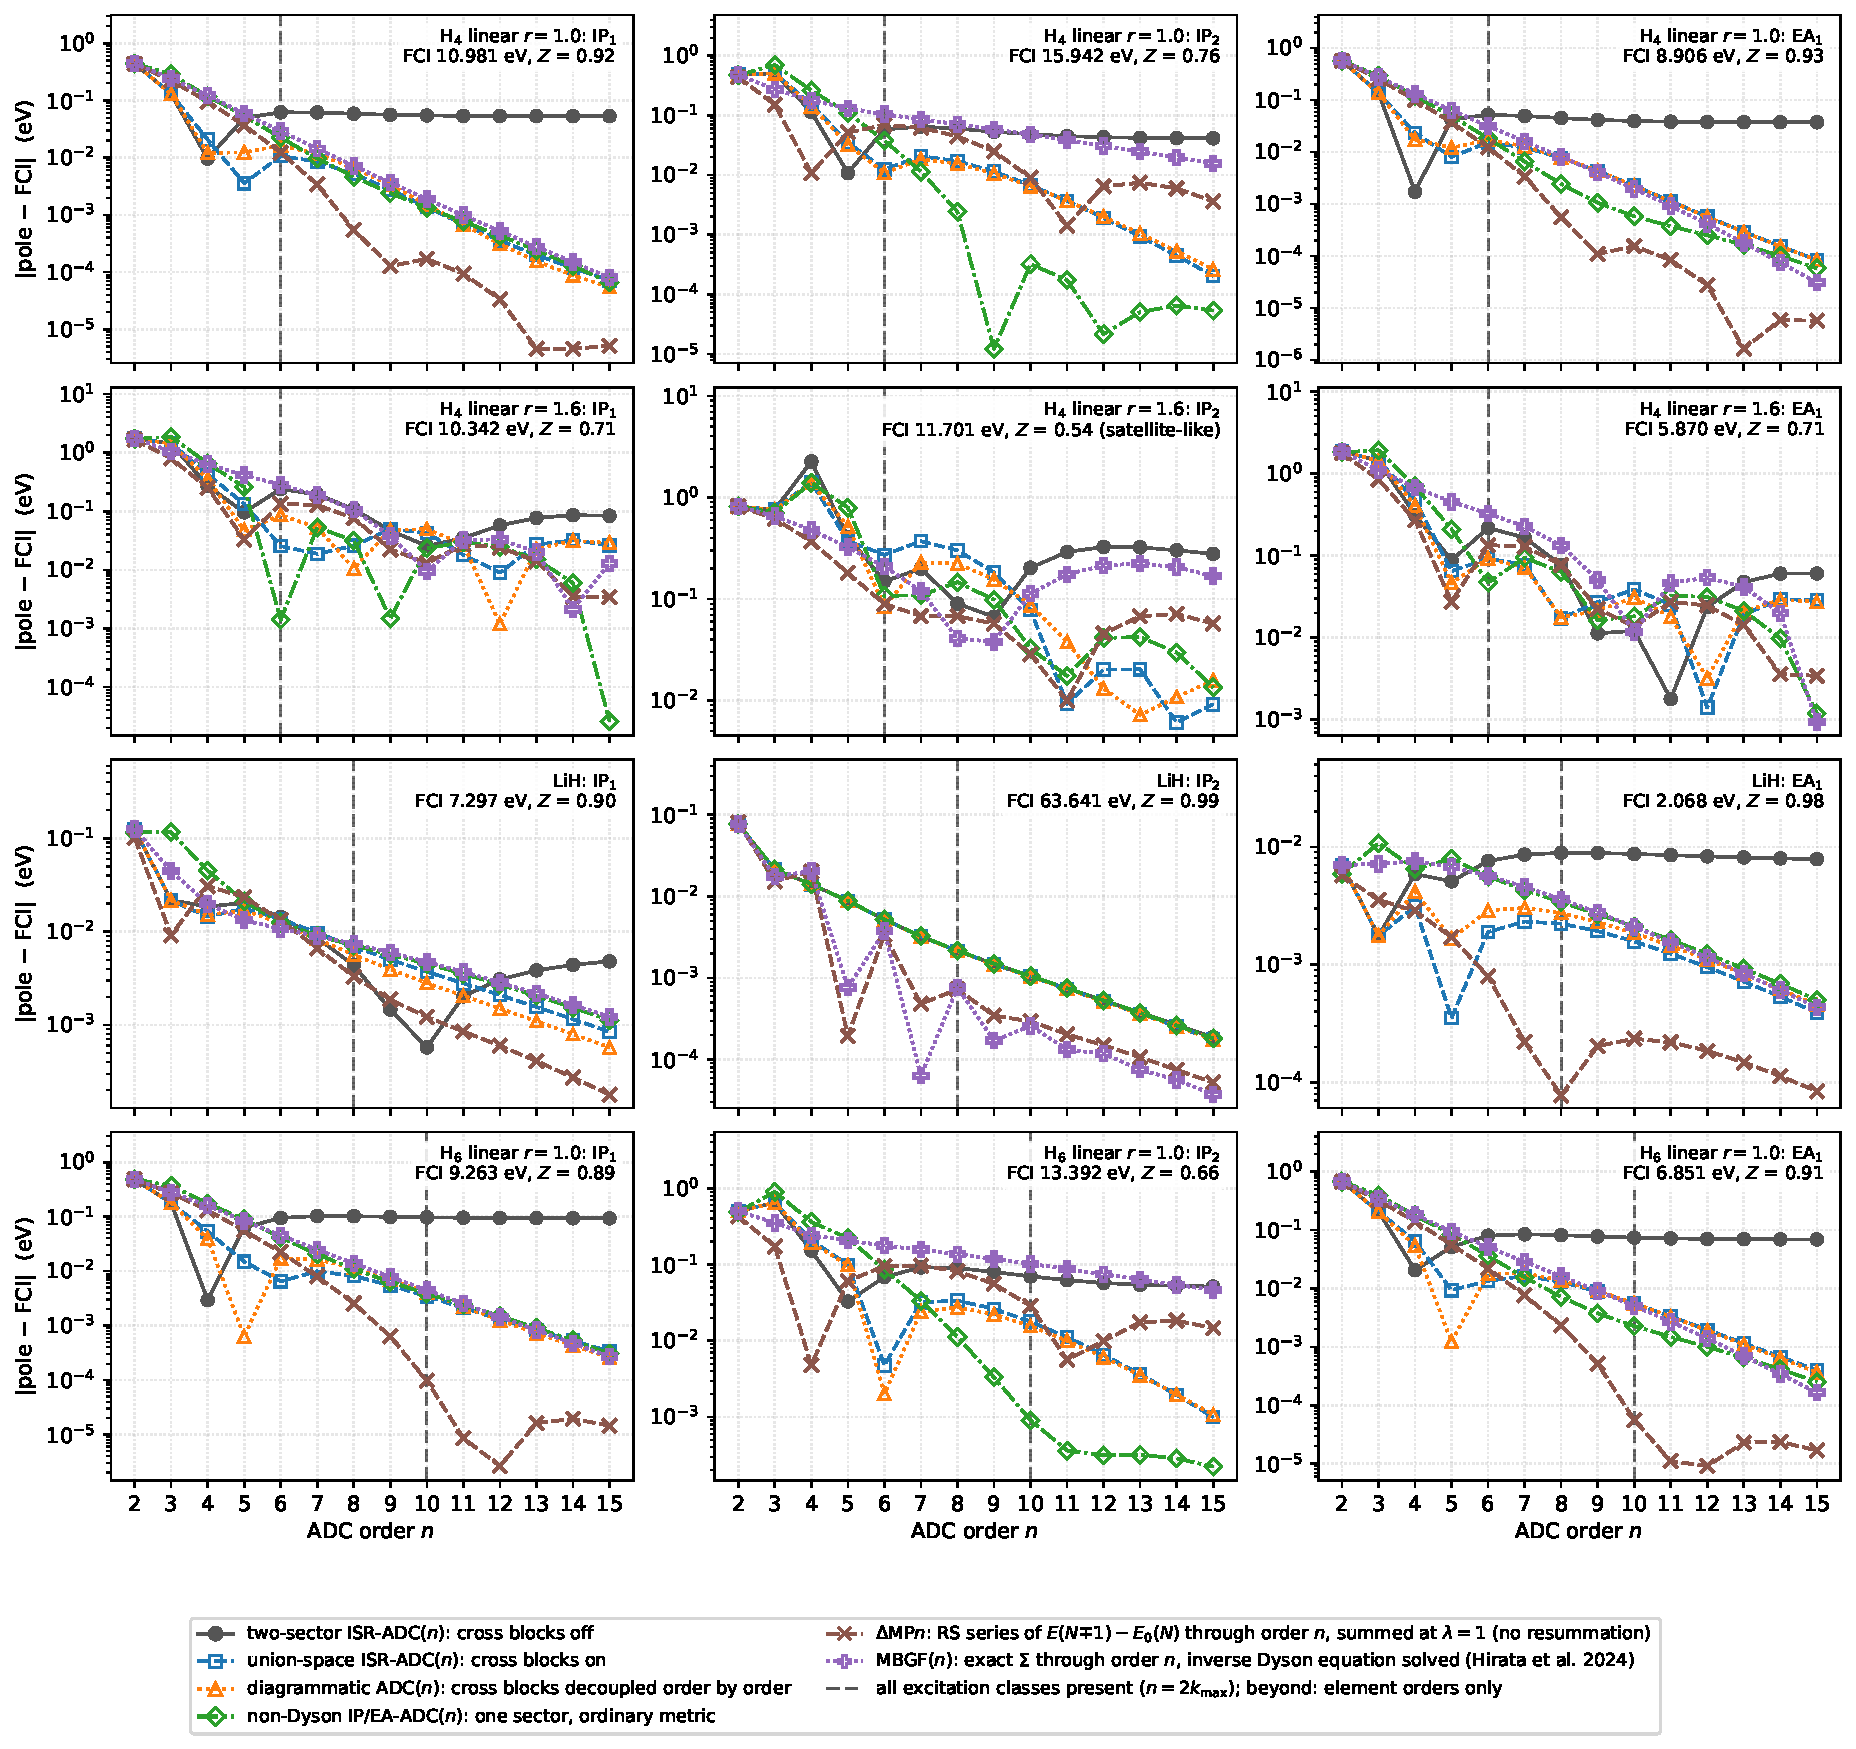
\includegraphics[width=\textwidth]{ip_convergence.pdf}
\caption{Principal ADC($n$) poles against FCI at $\la=1$. Dashed line: $n=2k_{\max}$, beyond which the
manifold is complete (for LiH the non-Dyson IP sector is complete at $n=6$).}
\label{fig:ip}
\end{figure*}

\section{Intermediate-state blocks}
\label{sec:blocks}

The excitation operators of the two sectors are the ionizing strings
\begin{equation}
\{\hat r^{-}_\nu\} = \{\cre{b}\ani{j}\ani{i},\ \cre{c}\cre{b}\ani{k}\ani{j}\ani{i},\ \ldots\}
\end{equation}
of sector I and the attaching strings
\begin{equation}
\{\hat r^{+}_\nu\} = \{\cre{a}\cre{b}\ani{j},\ \cre{a}\cre{b}\cre{c}\ani{k}\ani{j},\ \ldots\}
\end{equation}
of sector II. The ADC supermatrix is labelled by the single-character manifold
\begin{equation}
\{\hat X_J\} = \{\cre{p}\}\cup\{\hat r^{+}_\nu\}\cup\{\hat r^{-\dagger}_\nu\} ,
\end{equation}
in which every operator adds one electron. It is ordered into classes $k$: $\cre{p}$ is class 0; class $k$
holds the $(k{+}1)$p$k$h strings of sector II and the adjoints of the $(k{+}1)$h$k$p strings of sector I. Each $\hat X_J$ becomes the vector pair
$(\hat X_J\Psi_0,\hat X_J^\dagger\Psi_0)$ in $\mathcal H_{N+1}\oplus\mathcal H_{N-1}$, so that
\begin{equation}
\bbS_{IJ} = \langle\hat X_I\Psi_0|\hat X_J\Psi_0\rangle + \langle\hat X_J^\dagger\Psi_0|\hat X_I^\dagger\Psi_0\rangle
\end{equation}
is the metric $\langle\{\hat X_I^\dagger,\hat X_J\}\rangle$ and
\begin{equation}
\bbM_{IJ} = \langle\hat X_I\Psi_0|\hat H{-}E_0|\hat X_J\Psi_0\rangle
- \langle\hat X_J^\dagger\Psi_0|\hat H{-}E_0|\hat X_I^\dagger\Psi_0\rangle
\label{eq:M}
\end{equation}
is the superoperator $\langle\{\hat X_I^\dagger,[\hat H,\hat X_J]\}\rangle$. Inserting the RS series gives
$\bbS^{(m)}$ and $\bbM^{(m)}$ exactly. The intermediate states\cite{Schirmer_1991,Mertins_1996,Schirmer_2018}
follow from Gram--Schmidt of class $k$ against all lower classes and L\"owdin orthonormalization within
it, both done on the power series. The orthonormal supermatrix is
\begin{equation}
\tM =
\begin{pmatrix}
\bm\eps+\bm\Sigma(\infty) & \mathbf U^{\I} & \mathbf U^{\II} \\
\mathbf U^{\I\dagger} & -\mathbf K^{\I}-\mathbf C^{\I} & \mathbf X \\
\mathbf U^{\II\dagger} & \mathbf X^\dagger & \mathbf K^{\II}+\mathbf C^{\II}
\end{pmatrix} ,
\end{equation}
where $\mathbf K$ is the diagonal zeroth order and $\mathbf X$ the cross block between the sectors (its
metric counterpart vanishes identically). The inner projection\cite{tarantelli1992configuration}
$\mathbf G=[\bbS(\omega\bbS-\bbM)^{-1}\bbS]_{00}$ then has the Dyson form with
\begin{equation}
\bm\Sigma(\omega) = \bm\Sigma(\infty) + \mathbf U(\omega-\tM_{\rm cc})^{-1}\mathbf U^\dagger ,
\end{equation}
$\tM_{\rm cc}$ being all classes $k\ge1$. Over the complete manifold this reproduces FCI to $10^{-13}$.
Folded order by order, the dynamic part $\bm\Sigma_{\rm dyn}=\bm\Sigma-\bm\Sigma(\infty)$ is
\begin{equation}
\bm\Sigma^{(m)}_{\rm dyn}(\omega) = \sum_{a+b+c=m}\mathbf U^{(a)}\,\mathbf R^{(b)}(\omega)\,\mathbf U^{(c)\dagger} ,
\end{equation}
where $\mathbf R^{(b)}$ is the order-$b$ coefficient of $(\omega-\tM_{\rm cc})^{-1}$. This is the exact
Taylor reference; it agrees with the contour coefficients to $5\times10^{-13}$. ADC($n$)\cite{Schirmer_1982,Schirmer_1983}
keeps classes $k\le\lfloor n/2\rfloor$ and block $(k,l)$ through order $n-k-l$,
\begin{equation}
\big[\tM_{{\rm ADC}(n)}\big]_{kl} = \sum_{m=0}^{n-k-l}\tM^{(m)}_{kl} .
\label{eq:rule}
\end{equation}
Its eigenvalues at $\la=1$ are the poles; principal poles have orbital weight $Z>0.3$. For $n\ge n_{\rm c}$
(Table~\ref{tab:systems}) the manifold is complete and higher $n$ only adds orders to its matrix elements.

\section{Constructions}

All Dyson variants share $\bm\Sigma(\infty)$, $\mathbf U$ and the same-sector blocks exactly; they differ in
$\mathbf X$.

\begin{table}[hbt!]
\caption{The constructions of Fig.~\ref{fig:ip}. Limit: complete manifold, all orders.}
\label{tab:methods}
\begin{tabular}{lccc}
\hline\hline
construction & $\mathbf X$ & exact through & limit \\
\hline
two-sector ADC($n$) & dropped & $\la^3$ & not FCI \\
union ADC($n$) & Eq.~\eqref{eq:rule} & $\la^n$ & FCI \\
diagrammatic ADC($n$) & rotated & $\la^n$ & FCI \\
non-Dyson ADC($n$) & none & $\la^n$ & FCI \\
$\Delta$MP$n$ & -- & $\la^n$ & RS series \\
MBGF($n$) & -- & $\bm\Sigma$ to $\la^n$ & Dyson root \\
\hline\hline
\end{tabular}
\end{table}

\subsection{Union-space ISR-ADC(\texorpdfstring{$n$}{n})}

Union-space ISR-ADC($n$) keeps $\mathbf X$ under the rule of Eq.~\eqref{eq:rule}. The block between class
$k$ of sector I and class $l$ of sector II starts at order
\begin{equation}
L_{kl} = \Big\lceil\frac{k+l+1}{2}\Big\rceil ,
\end{equation}
so under the rule the block $\mathbf X_{11}$ enters at $n=4$, $\mathbf X_{12}$ at $n=5$, $\mathbf X_{22}$
and $\mathbf X_{13}$ at $n=7$, $\mathbf X_{23}$ at $n=8$ and $\mathbf X_{33}$ at $n=10$. With these blocks
the fold is exact through $\la^n$ at every $n$ tested ($n=4$--9, to $10^{-12}$).

\subsection{Two-sector ISR-ADC(\texorpdfstring{$n$}{n}) and the cross block}
\label{sec:twosector}
Two-sector ISR-ADC($n$) orthonormalizes and folds each sector on its own,
and thus yields the familiar form of the self-energy,
organized by $+$ and $-$ branches,
\begin{equation}
\bm\Sigma(\omega) = \bm\Sigma(\infty)
+ \mathbf U^{\II}\big(\omega-\mathbf K^{\II}-\mathbf C^{\II}\big)^{-1}\mathbf U^{\II\dagger}
+ \mathbf U^{\I}\big(\omega+\mathbf K^{\I}+\mathbf C^{\I}\big)^{-1}\mathbf U^{\I\dagger} .
\label{eq:twosector}
\end{equation}
Its blocks are exactly the same-sector blocks of $\tM$, so it is $\tM$ with $\mathbf X$ deleted. The cross
block vanishes at the two lowest orders,
\begin{equation}
\mathbf X^{(0)} = \mathbf X^{(1)} = 0 ,
\end{equation}
but not at second, where it is a contraction of the first-order doubles with the two-electron integrals.
Expanding the union fold in $\mathbf X$, the leading term the two-sector construction misses is
\begin{equation}
\Delta\bm\Sigma^{(4)} = \mathbf U^{\I(1)}\big(\omega+\mathbf K^{\I}_1\big)^{-1}\mathbf X^{(2)}_{11}
\big(\omega-\mathbf K^{\II}_1\big)^{-1}\mathbf U^{\II(1)\dagger} + \mathrm{h.c.} ,
\label{eq:defect}
\end{equation}
which matches the $\la^4$ difference of the two folds to $5\times10^{-18}$. Two-sector ISR-ADC($n$) is
therefore exact only through $\la^3$, for every $n$.

The defect is fundamental, its complete-manifold limit is not FCI.
as can be seen clearly in Fig.~\ref{fig:ip}.
This obstacle has been identified by Tarantelli and Cederbaum.\cite{tarantelli1992configuration} They write the
Dyson equation as a configuration-interaction problem in $\mathcal H_{N+1}\oplus\mathcal H_{N-1}$, with a
composite Hamiltonian that is $\bbM$ of Eq.~\eqref{eq:M}. The block that couples the $(N+1)$ and $(N-1)$
configurations vanishes in zeroth and first order but not in second, and they conclude that this coupling
``prevents the possibility of reproducing analytically the fourth-order ADC scheme'', since ADC assumes that
the self-energy splits into independent $(N+1)$ and $(N-1)$ parts. They remove the coupling by a further
unitary transformation that block-diagonalizes the configuration space. This transformation can only be
built order by order, and with an exactly solvable two-electron example they show that no transformation
built from the ground state alone achieves the decoupling. The two-sector ISR is built from the ground state
alone and is decoupled by construction.

\subsection{Diagrammatic ADC(\texorpdfstring{$n$}{n})}
\label{sec:diagrammatic}

Diagrammatic ADC($n$) removes $\mathbf X$ by the Tarantelli--Cederbaum
rotation\cite{tarantelli1992configuration} $\mathbf W=e^{\mathbf A}$, with $\mathbf A$ antisymmetric in the
I--II blocks and
\begin{equation}
A^{(m)}_{\mu\nu} = \frac{R^{(m)}_{\mu\nu}}{K_\nu-K_\mu} ,
\end{equation}
$\mathbf R^{(m)}$ being the I--II part of $[\mathbf W^\intercal\tM\mathbf W]^{(m)}$ from
$\mathbf A^{(<m)}$; Eq.~\eqref{eq:rule} is applied to the rotated blocks. At third order this moves
$\mathbf X^{(2)}$ into the couplings,
\begin{equation}
\delta U^{\II(3)}_{p\nu} = \sum_{\mu\in\I_1}\frac{U^{\I(1)}_{p\mu}X^{(2)}_{\mu\nu}}{K_\nu-K_\mu} ,
\end{equation}
where $K_\nu-K_\mu$ is a 3p3h energy; these rows reproduce the diagrammatic ADC(4)
rows\cite{Schirmer_1983} to $10^{-18}$.

\subsection{Non-Dyson ADC(\texorpdfstring{$n$}{n})}

Non-Dyson ADC($n$)\cite{Schirmer_1998,Trofimov_2005}
builds the ISR from $\hat r^{-}_\nu\Psi_0$ in $\mathcal H_{N-1}$ (or $\hat r^{+}_\nu\Psi_0$ in
$\mathcal H_{N+1}$) with the ordinary overlap and the same rule; its eigenvalues are the IPs (EAs).

\subsection{Perturbative references}

$\Delta$MP$n$ is the RS series of $E_{N-1}(\la)-E_0(\la)$ for the Koopmans-connected state, summed through
order $n$. MBGF($n$)\cite{Hirata_2024} takes the exact $\bm\Sigma^{[n]}=\sum_{m\le n}\bm\Sigma^{(m)}$
and solves
\begin{equation}
\omega = e_p(\omega) ,
\end{equation}
with $e_p$ the eigenvalue of $\bm\eps+\bm\Sigma^{[n]}(\omega)$ of largest weight on $p$, taking the root of
largest residue. The pole Taylor series of union, diagrammatic and non-Dyson ADC($n$) equal the exact one
through $\la^n$ to $10^{-17}$ ($n\le15$); the two-sector pole deviates from $\la^4$ on.

\section{Ne and Ar beyond ADC(5)}
\label{sec:neon}

Fig.~\ref{fig:neon} follows the non-Dyson ADC($n$) series of the Ne and Ar valence ionizations in
correlation-consistent bases to high order, against the FCI IP of the same block. The series are the
exact symmetry-adapted ones of the $\la$-scaled problem of the previous sections, so no
approximation enters beyond the basis: Ne/cc-pVDZ ($1s$ frozen) through $n=9$, Ne/aug-cc-pVDZ ($1s$ frozen) and
Ar/aug-cc-pVDZ ($1s2s2p$ frozen) through $n=7$. ADC(1) is Koopmans' theorem. The lower row zooms on
$n\ge5$. The error of the Ne/aug-cc-pVDZ series is still $+0.09$ and $+0.13$\,eV at $n=7$ for
$2p$ and $2s$: in a diffuse basis the series itself converges slowly, and this is what the
ADC(5) errors of Figs.~\ref{fig:fcadz1}--\ref{fig:fcadz3} contain.

\begin{figure*}[hbt!]
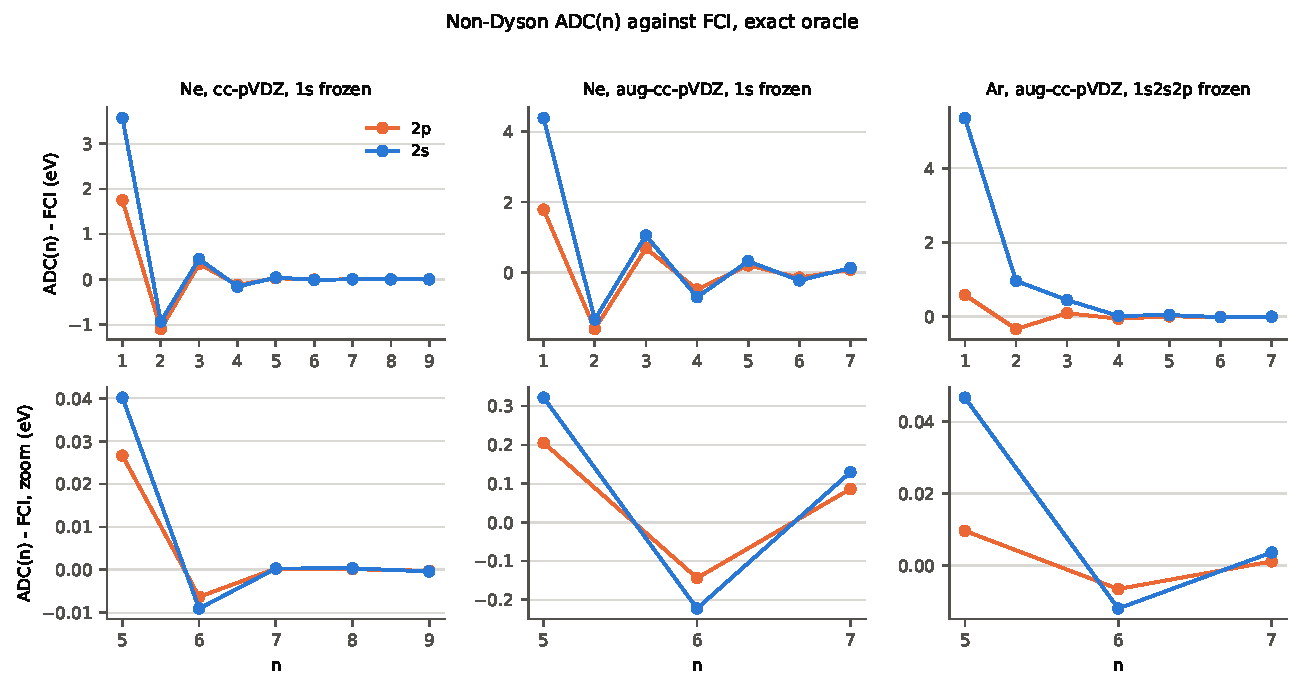
\includegraphics[width=\textwidth]{oracle_ne_ar_convergence.pdf}
\caption{Non-Dyson ADC($n$) IP minus the FCI IP of Ne/cc-pVDZ, Ne/aug-cc-pVDZ and Ar/aug-cc-pVDZ
(frozen core as stated in the text). Top: $n=1$ (Koopmans) to the last order; bottom: $n\ge5$.}
\label{fig:neon}
\end{figure*}

\section{Dyson ADC(2)--(5) for molecules}
\label{sec:molecules}

Figs.~\ref{fig:fcadz1}--\ref{fig:fcadz3} show the errors of Dyson diagrammatic ADC($n$) IP for $n=2$--5 
(frozen core; aug-cc-pVDZ) against selected CI (sCI) value of the same basis, and the convergence of CC is shown for comparison.
The mean absolute ADC(5) error of the 24 states shown at the time of writing is 0.34\,eV, against 0.04\,eV for CCSDT.
For most states the error alternates in sign with $n$ and does not decrease monotonically.

\begin{figure*}[hbt!]
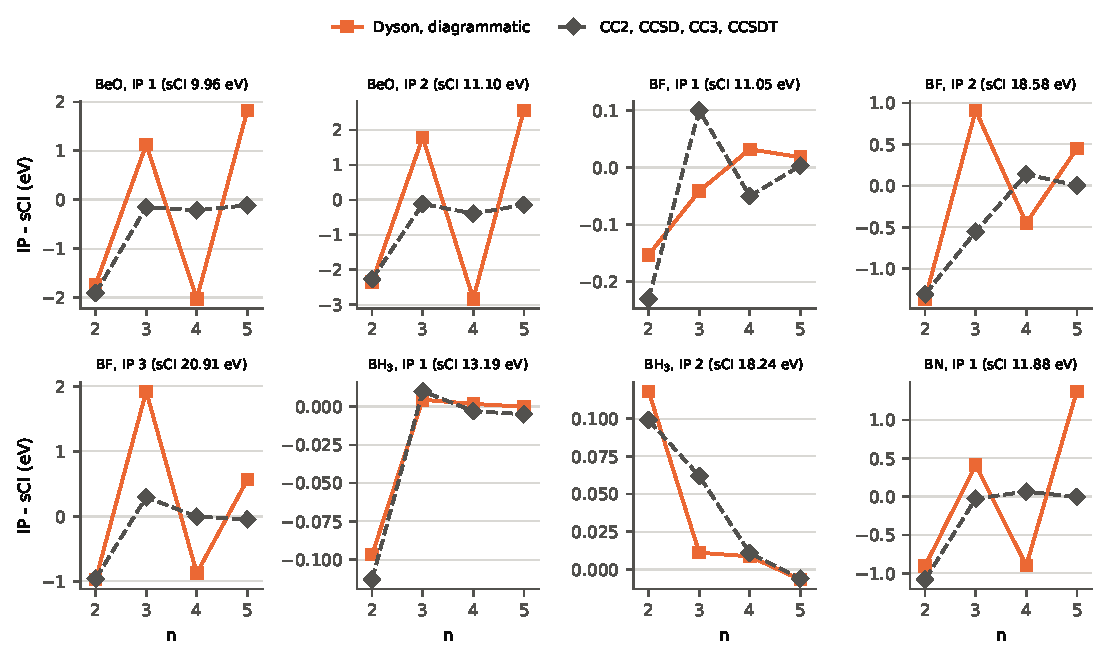
\includegraphics[width=0.8\textwidth]{fc_adz_diagcc_part1.pdf}
\caption{Dyson diagrammatic ADC($n$) IP and coupled cluster minus the sCI IP, frozen core, aug-cc-pVDZ (1/3).}
\label{fig:fcadz1}
\end{figure*}

\begin{figure*}[hbt!]
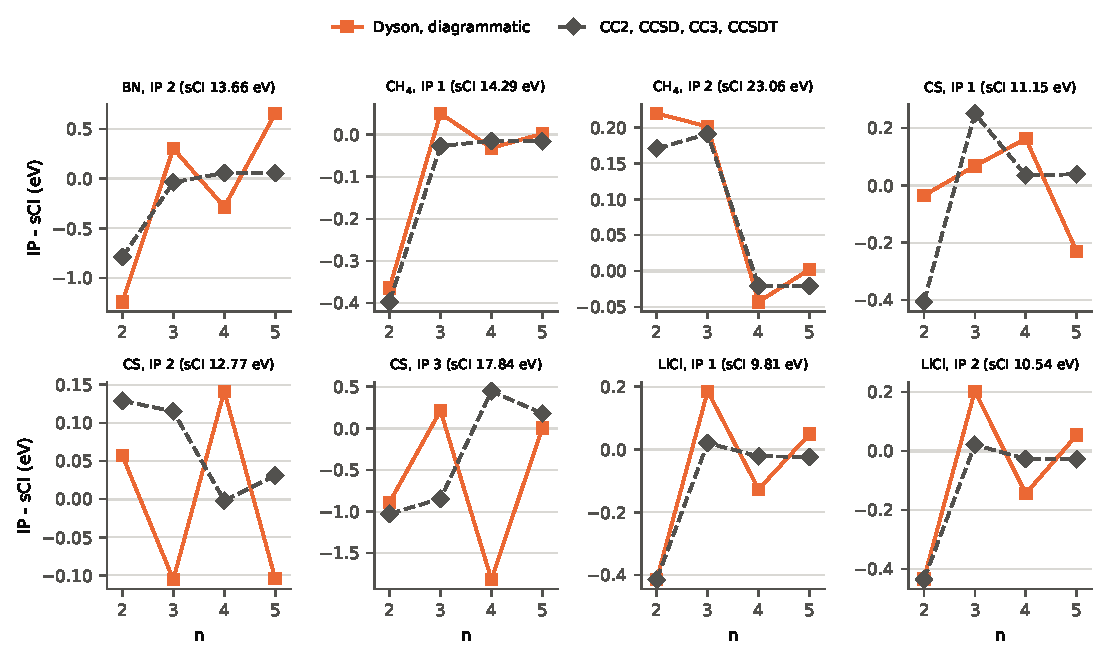
\includegraphics[width=0.8\textwidth]{fc_adz_diagcc_part2.pdf}
\caption{As Fig.~\ref{fig:fcadz1} (2/3).}
\label{fig:fcadz2}
\end{figure*}

\begin{figure*}[hbt!]
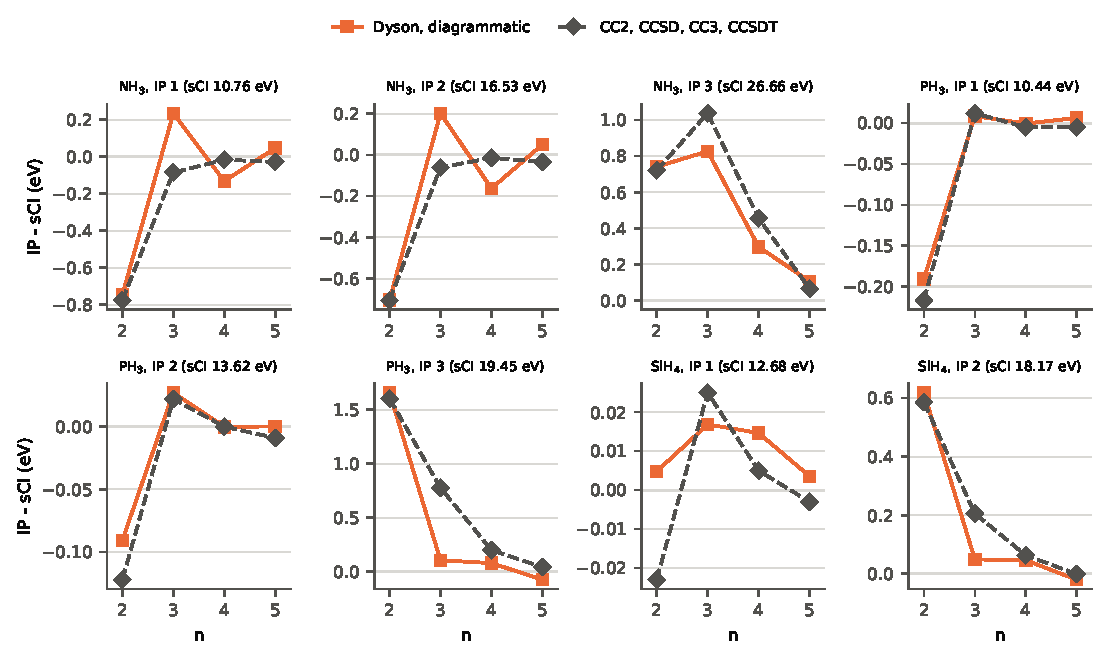
\includegraphics[width=0.8\textwidth]{fc_adz_diagcc_part3.pdf}
\caption{As Fig.~\ref{fig:fcadz1} (3/3).}
\label{fig:fcadz3}
\end{figure*}

\bibliography{isr_adc_numerics}

\end{document}
